%% =====================================================================
%% EnsFlow — NeurIPS 2026 draft (work in progress)
%%
%% Compile:
%%   pdflatex main && bibtex main && pdflatex main && pdflatex main
%%
%% NOTE: neurips_2026.sty is not bundled. For now we use article + the
%% neurips-like formatting below. Drop in the official style file and
%% replace the \documentclass line once it's available.
%% =====================================================================

\documentclass{article}

\usepackage[margin=1.25in]{geometry}
\usepackage{times}
\usepackage{microtype}

\usepackage{amsmath, amssymb, amsthm, mathtools}
\usepackage{graphicx}
\usepackage{booktabs}
\usepackage{multirow}
\usepackage{xcolor}
\usepackage{enumitem}
\usepackage{bm}
\usepackage{url}
\usepackage{natbib}
\usepackage{tikz}
\usetikzlibrary{arrows.meta, calc, positioning, fit, backgrounds}
\usepackage[colorlinks, linkcolor=blue!50!black, citecolor=blue!50!black, urlcolor=blue!50!black]{hyperref}

% ---- Theorem environments --------------------------------------------------
\newtheorem{proposition}{Proposition}
\newtheorem{lemma}{Lemma}
\newtheorem{theorem}{Theorem}
\newtheorem{corollary}{Corollary}
\theoremstyle{remark}
\newtheorem{remark}{Remark}
\theoremstyle{definition}
\newtheorem{assumption}{Assumption}

% ---- Macros ---------------------------------------------------------------
\newcommand{\R}{\mathbb{R}}
\newcommand{\E}{\mathbb{E}}
\newcommand{\Var}{\mathrm{Var}}
\newcommand{\Cov}{\mathrm{Cov}}
\newcommand{\tr}{\mathrm{tr}}
\newcommand{\SO}{\mathrm{SO}}
\newcommand{\SE}{\mathrm{SE}}
\newcommand{\so}{\mathfrak{so}}
\newcommand{\Log}{\mathrm{Log}}
\newcommand{\Exp}{\mathrm{Exp}}
\newcommand{\sigmoid}{\sigma_{\mathrm{sig}}}
\DeclareMathOperator*{\argmin}{arg\,min}
\DeclareMathOperator*{\argmax}{arg\,max}
\newcommand{\todo}[1]{\textcolor{red}{\textbf{[TODO: #1]}}}

% ---- Title block ----------------------------------------------------------
\title{\textsc{EnsFlow}: Self-Regulating Heteroscedastic Bridges on $\SE(3)$\\
for RNA Conformational Ensemble Generation}

\author{%
  Anonymous Authors\\
  Anonymous Institution\\
  \texttt{anonymous@example.com}%
}

\date{}

\begin{document}
\maketitle

% =========================================================================
\begin{abstract}
Modeling the conformational ensembles of RNA is a central open problem in
machine learning for structural biology: RNA function often arises from
multi-state flexibility rather than a single native fold, yet every modern
structure-prediction system, including the RNA branch of AlphaFold3, outputs
a single point estimate. We introduce \textsc{EnsFlow}, a three-level
hierarchical framework for RNA ensemble generation on $\SE(3)^L$ built around
a \emph{conditional heteroscedastic stochastic bridge}. The central object is
a residue-wise, state-dependent bridge width field whose modulation is learned
jointly with an $\SE(3)$ flow-matching drift. Our key methodological
contribution is a \emph{self-regulating} training objective: we supervise the
bridge width via a heteroscedastic Gaussian negative log-likelihood of the
drift model's own residual, and prove that its closed-form optimum is
$\sigma^{\ast}=\|r\|$---the bridge width at any $(t,i)$ is exactly the drift
model's residual magnitude at that point. This yields a temperature-free,
self-calibrating uncertainty signal that ties stochastic exploration directly
to model reliability, and admits a Bayesian interpretation as the trace of the
posterior covariance of the clean state given the noisy state. We further
introduce \emph{B-factor anchoring}, a supervision signal that aligns the
learned uncertainty field with experimentally measured atomic displacement
parameters---to our knowledge the first direct link between ML epistemic
uncertainty and crystallographic aleatoric flexibility in an $\SE(3)$
generative model. We prove that Level~1 (deterministic flow matching) and the
fixed-width stochastic bridge both arise as strict degenerate limits of Level~2,
giving a clean hierarchy. \todo{Empirical results on RNA ensemble benchmarks.}
\end{abstract}

% =========================================================================
\section{Introduction}
\label{sec:intro}

\paragraph{RNAs are not rigid.}
Unlike most proteins, where a single ``native'' fold captures the dominant
functional state, many RNAs function precisely through conformational
heterogeneity: riboswitches undergo ligand-induced structural
switches~\citep{serganov2013decade}, ribozymes traverse distinct catalytic
states, and regulatory RNAs adopt transient interaction-competent
folds~\citep{mustoe2014hierarchy}. Representing an RNA with a single structure
fundamentally misses this functional machinery. Yet every modern structure
prediction system---including the RNA module of AlphaFold3~\citep{alphafold3}
---outputs a single point estimate, leaving conformational \emph{ensemble}
generation as one of the most consequential open problems in machine learning
for RNA structural biology.

\paragraph{What existing $\SE(3)$ generative models miss.}
Recent progress on $\SE(3)$-equivariant generative models for biomolecular
backbones has been rapid. FrameDiff~\citep{framediff} and
FrameFlow~\citep{frameflow} established $\SE(3)$ diffusion and flow matching
for protein backbones; FoldFlow and its stochastic variant
FoldFlow-SFM~\citep{foldflow} extended flow matching to stochastic bridges on
$\SE(3)$ and observed that stochasticity improves novelty and diversity. For
RNA, RNA-FrameFlow~\citep{rnaframeflow} adapted this to nucleotide frames.
Ensemble-focused methods---Distributional Graphormer (DiG)~\citep{dig},
BioEmu~\citep{bioemu}, AlphaFlow~\citep{alphaflow}, and
Str2Str~\citep{str2str}---apply similar ideas to \emph{protein} ensembles.
Strikingly absent from all of these: any mechanism to learn \emph{where} and
\emph{how much} stochasticity to inject. FoldFlow-SFM uses a global
time-dependent schedule $\sigma(t)$; DiG and BioEmu use fixed diffusion
coefficients; AlphaFlow reuses a flow-matching schedule with no local
adaptation. The stochasticity is global and state-agnostic---the same amount
of noise at every residue regardless of whether that residue sits in a stable
stem or a flexible loop.

\paragraph{The key insight.}
RNA flexibility is emphatically not global. A hairpin has rigid base-paired
stems and flexible apical loops; a riboswitch aptamer is stable while its
expression platform is dynamic; many tRNAs have one stable core and one mobile
anticodon arm. Uniform noise erases this signal. What we want is a
\emph{learned heteroscedastic uncertainty field} on $\SE(3)^L$ that assigns
local stochasticity where the model itself is uncertain, not a single global
temperature. This raises two questions:
\begin{itemize}[leftmargin=2em,itemsep=0pt,topsep=2pt]
\item[(i)] What training signal should guide such a field?
\item[(ii)] Does the learned field correspond to anything physically measurable?
\end{itemize}
We answer both. \emph{First}, we show that the bridge width maximizing the
likelihood of the drift model's own residual is the residual magnitude
itself---yielding a closed-form, temperature-free, self-regulating objective
(\S\ref{subsec:nll}, Prop.~\ref{prop:self-reg}). This ties stochastic
exploration to model reliability: \emph{the model is more stochastic exactly
where it is less certain about the clean structure}. \emph{Second}, we show
that supervising the learned bridge width with experimental B-factors
(crystallographic atomic displacement parameters) aligns it with physically
measured flexibility, giving a concrete, falsifiable connection between model
epistemic uncertainty and experimental aleatoric flexibility
(\S\ref{subsec:bfactor}).

\paragraph{Contributions.}
\begin{enumerate}[leftmargin=1.6em,itemsep=2pt,topsep=3pt]
\item \textbf{\textsc{EnsFlow} framework.} A three-level hierarchical model for
RNA ensemble generation on $\SE(3)^L$: Level~1 (deterministic flow matching),
Level~2 (conditional heteroscedastic stochastic bridge), Level~3 (bridge with
B-factor anchoring). We prove that Level~1 and fixed-width FoldFlow-SFM-style
bridges arise as strict degenerate limits of Level~2
(Prop.~\ref{prop:degenerate}).

\item \textbf{Self-regulating NLL objective.} A heteroscedastic Gaussian NLL
loss on the drift residual whose closed-form pointwise minimum is
$\sigma^{\ast}=\|r\|$ (Prop.~\ref{prop:self-reg}). Under a Bayes-optimal drift
assumption, this corresponds to the trace of the posterior covariance of the
clean state given the noisy state (Cor.~\ref{cor:posterior}). No temperature,
no KL weight, no hand-tuned balance between exploration and fidelity.

\item \textbf{B-factor physical anchoring.} A novel supervision signal aligning
the learned bridge width with experimentally measured B-factors, providing the
first direct link between generative-model epistemic uncertainty and physical
flexibility measurements in an $\SE(3)$ framework.

\item \textbf{Empirical validation.} On \todo{RNA ensemble benchmarks}, we show
\todo{improvements in} ensemble coverage, diversity, and physical validity
over deterministic and fixed-width bridge baselines, with the learned
uncertainty field exhibiting significant Spearman correlation against held-out
B-factors---even when B-factor supervision is disabled (Level~2).
\end{enumerate}

% =========================================================================
\section{Related Work}
\label{sec:related}

Table~\ref{tab:related} places EnsFlow against representative prior work along
the axes that matter for our contribution.

\begin{table}[t]
\centering
\small
\caption{Positioning of \textsc{EnsFlow} against representative prior work on
$\SE(3)$ generative modeling and ensemble generation. ``SDE'' = stochastic
dynamics; ``Learned $\sigma$'' = noise coefficient learned jointly with drift;
``State-dep.'' = noise depends on current noisy state; ``Residue-wise'' = noise
varies per residue; ``Physical anchor'' = learned uncertainty explicitly tied
to experimentally measured flexibility. \textsc{EnsFlow} is the first to check
all boxes.}
\label{tab:related}
\begin{tabular}{lcccccl}
\toprule
Method & SDE? & Learned $\sigma$ & State-dep.\ & Residue-wise & Phys.\ anchor & Target \\
\midrule
FrameDiff~\citep{framediff} & diffusion & fixed & -- & -- & -- & protein \\
FrameFlow~\citep{frameflow} & ODE & -- & -- & -- & -- & protein \\
RNA-FrameFlow~\citep{rnaframeflow} & ODE & -- & -- & -- & -- & RNA \\
FoldFlow-SFM~\citep{foldflow} & \checkmark & fixed $\sigma(t)$ & -- & -- & -- & protein \\
AlphaFlow~\citep{alphaflow} & $\approx$ & fixed schedule & -- & -- & -- & protein ens.\ \\
DiG~\citep{dig} & diffusion & fixed & -- & -- & -- & protein ens.\ \\
BioEmu~\citep{bioemu} & ODE/SDE & fixed & -- & -- & -- & protein ens.\ \\
Str2Str~\citep{str2str} & diffusion & fixed & -- & -- & -- & protein ens.\ \\
Improved DDPM~\citep{improveddpm} & diffusion & \checkmark (VLB) & -- & iso.\ pixel & -- & images \\
\midrule
\textbf{EnsFlow (ours)} & \checkmark & \checkmark (NLL) & \checkmark & \checkmark & \checkmark & \textbf{RNA ens.} \\
\bottomrule
\end{tabular}
\end{table}

\paragraph{$\SE(3)$ flow/diffusion for biomolecules.}
FrameDiff~\citep{framediff}, FrameFlow~\citep{frameflow}, Chroma~\citep{chroma},
Genie~\citep{genie}, and RFdiffusion~\citep{rfdiffusion} place equivariant
generative models directly on $\SE(3)^L$ using either diffusion or flow
matching. All use global, fixed noise schedules. RNA-FrameFlow~\citep{rnaframeflow}
is the closest single-structure antecedent for our target domain; EnsFlow
builds on its backbone architecture and $\SE(3)$ flow-matching drift.

\paragraph{Stochastic bridges and interpolants.}
FoldFlow-SFM~\citep{foldflow} replaces deterministic flow paths with $\SE(3)$
stochastic bridges, using translation Brownian bridges and SO(3) IGSO(3)
approximations. Stochastic interpolants~\citep{stochasticinterpolants} and
Schr\"odinger bridge matching~\citep{shi2023dsbm} provide the broader theoretical
frame. In all of these, the diffusion coefficient is a fixed function of
$t$---never residue-wise and never state-dependent. Our Level~2 is a strict
generalization (Prop.~\ref{prop:degenerate}).

\paragraph{Ensemble generation for biomolecules.}
DiG~\citep{dig}, BioEmu~\citep{bioemu}, AlphaFlow~\citep{alphaflow}, and
Str2Str~\citep{str2str} generate protein conformational ensembles, typically
trained on MD trajectories or multi-state experimental data. RNA-specific
ensemble generation has received much less attention; we are not aware of a
published ML method targeting RNA conformational ensembles with
residue-resolved flexibility.

\paragraph{Learned variance in generative modeling.}
Improved DDPM~\citep{improveddpm} learns variance via a hybrid $L_{\text{simple}}
+\nobreak L_{\text{vlb}}$ loss; Variational Diffusion Models~\citep{vdm} learn
an SNR schedule. Both operate on Euclidean pixels and learn a single
time-indexed variance shared across all coordinates. Our per-residue,
state-dependent $\sigma$ on $\SE(3)^L$, trained by a simple NLL with closed-form
minimum at $\sigma^{\ast}=\|r\|$, is a different animal.

% =========================================================================
\section{Preliminaries}
\label{sec:prelim}

\paragraph{Nucleotide frames.}
Following~\citet{rnaframeflow}, we represent an RNA backbone of length $L$ as a
sequence of rigid frames $G=\{G_i\}_{i=1}^L$, $G_i=(x_i, R_i)\in\SE(3)$, where
$x_i\in\R^3$ is a reference atom position (C4$'$ for RNA) and $R_i\in\SO(3)$ is
a local frame constructed from neighboring atoms. Given sequence
$a=(a_1,\ldots,a_L)$, the generation task is to model
$p(G\mid a)$.

\paragraph{Time convention.}
Throughout, $t=0$ denotes the noise/prior end and $t=1$ denotes the clean data
end, so at training time we observe a clean $(x_1, R_1)$ and sample a noisy
intermediate $(x_t, R_t)$. The drift of a flow matching model predicts the
\emph{clean endpoint} $\hat{G}_{1\mid t}=(\hat{x}_{1\mid t},\hat{R}_{1\mid t})$;
the velocity is induced as
\begin{equation}
u^x(i,t)=\frac{\hat{x}_{i,1\mid t}-x_{i,t}}{1-t},\qquad
u^\omega(i,t)=\frac{1}{1-t}\,\Log\!\big(R_{i,t}^\top\hat{R}_{i,1\mid t}\big),
\label{eq:velocity}
\end{equation}
where $\Log:\SO(3)\to\so(3)\cong\R^3$ is the matrix logarithm
(rotation-vector) map.

\paragraph{$\SE(3)$ flow matching.}
The Level~1 drift is trained by the standard flow-matching MSE against the
ground-truth velocity field:
\begin{equation}
\mathcal{L}_{\text{flow}}=\E_{t,G_1,G_t}\!\Bigg[
  w_x\big\|u^x_\theta-u^{x,\ast}\big\|_2^2
  + w_\omega\big\|u^\omega_\theta-u^{\omega,\ast}\big\|_2^2
\Bigg],
\label{eq:flow-loss}
\end{equation}
with weights $w_x,w_\omega>0$ balancing translation (\AA) and rotation (rad).

\paragraph{$\SO(3)$ Brownian bridges via tangent-space Gaussians.}
For small angular variance, the IGSO(3) density of a rotation $R$ with
concentration $\sigma^2$ is well-approximated by the tangent-space Gaussian
$p(R\mid\sigma^2)\propto\exp\!\big(-\|\Log(R)\|^2/(2\sigma^2)\big)$; the
relative error in log-likelihood vanishes as $\sigma\to
0$~\citep{nikolayev1997igso3,leach2022denoisingso3}. We use this approximation
in \S\ref{subsec:nll}.

% =========================================================================
\section{Method}
\label{sec:method}

Our central object is a conditional heteroscedastic stochastic bridge on
$\SE(3)^L$. We first formalize the bridge and its parameterization
(\S\ref{subsec:bridge}), then introduce the self-regulating NLL objective
(\S\ref{subsec:nll}), the BridgeWidthNet that implements the modulation field
(\S\ref{subsec:bwnet}), and the B-factor anchor (\S\ref{subsec:bfactor}). We
conclude with the theoretical properties of the framework
(\S\ref{subsec:theory}). Figure~\ref{fig:architecture} gives a bird's-eye view
of the training-time data flow: a single flow-matching drift network shares
its outputs both with the flow loss and with a lightweight
\textsc{BridgeWidthNet} that predicts the per-residue stochastic bridge width.

% ---------------------------------------------------------------
\begin{figure}[t]
\centering
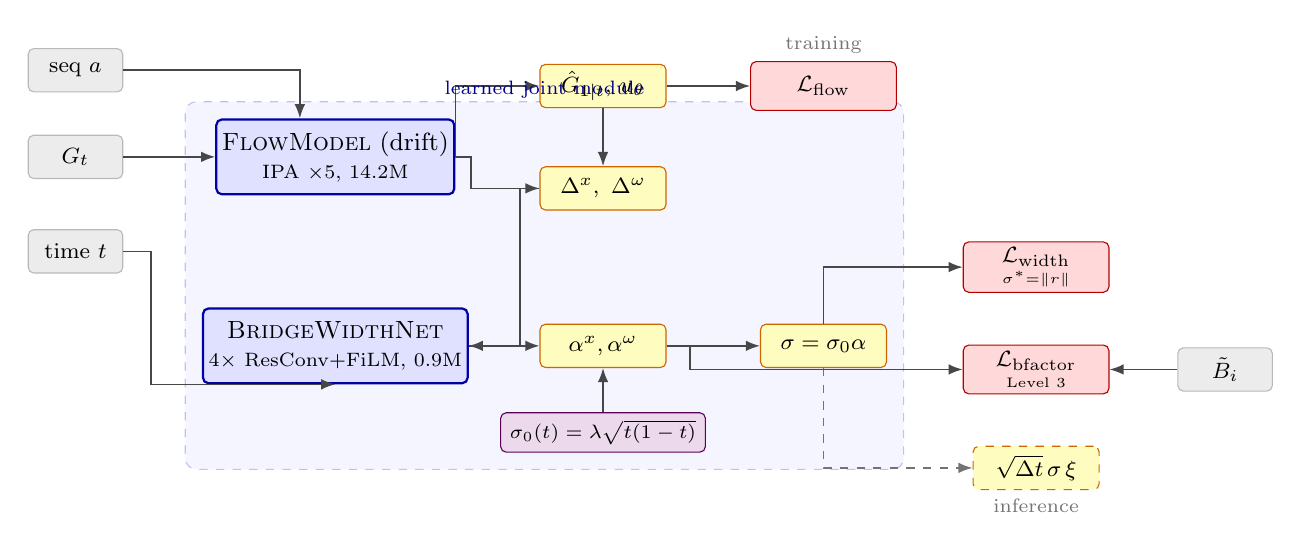
\begin{tikzpicture}[
  font=\small,
  >={Latex[length=1.8mm]},
  box/.style={draw, rounded corners=2pt, align=center, inner sep=2pt},
  net/.style={box, fill=blue!12, draw=blue!65!black, thick,
              minimum width=2.8cm, minimum height=0.95cm},
  inp/.style={box, fill=gray!15, draw=gray!55,
              minimum width=1.2cm, minimum height=0.55cm, font=\footnotesize},
  op/.style={box, fill=yellow!25, draw=orange!80!black,
             minimum width=1.6cm, minimum height=0.55cm, font=\footnotesize},
  loss/.style={box, fill=red!15, draw=red!70!black,
               minimum width=1.85cm, minimum height=0.62cm, font=\footnotesize},
  schd/.style={box, fill=violet!15, draw=violet!70!black,
               minimum width=2.6cm, minimum height=0.5cm, font=\scriptsize},
  grp/.style={rounded corners=4pt, inner sep=6pt},
  arr/.style={->, semithick, draw=black!72},
  darr/.style={->, semithick, dashed, draw=black!55},
]

% ============ NODES ============

% Inputs column
\node[inp] (seq) at (0, 2.1) {seq $a$};
\node[inp] (Gt)  at (0, 1.0) {$G_t$};
\node[inp] (tt)  at (0,-0.2) {time $t$};

% Drift network
\node[net] (drift) at (3.3, 1.0)
  {\textsc{FlowModel} (drift)\\[-1pt]\scriptsize IPA $\times 5$, 14.2M};

% Drift outputs (top row) and flow loss
\node[op]   (ghat)  at (6.7, 1.9) {$\hat G_{1|t},\, u_\theta$};
\node[loss] (Lflow) at (9.5, 1.9) {$\mathcal{L}_{\mathrm{flow}}$};

% Residual box (between rows, right of drift)
\node[op] (delta) at (6.7, 0.6) {$\Delta^x,\ \Delta^\omega$};

% BridgeWidthNet (bottom row)
\node[net] (bwnet) at (3.3,-1.4)
  {\textsc{BridgeWidthNet}\\[-1pt]\scriptsize 4$\times$ ResConv+FiLM, 0.9M};

% BridgeWidthNet outputs
\node[op]   (alpha) at (6.7,-1.4) {$\alpha^x,\alpha^\omega$};
\node[schd] (sig0)  at (6.7,-2.5) {$\sigma_0(t)=\lambda\sqrt{t(1-t)}$};
\node[op]   (sig)   at (9.5,-1.4) {$\sigma=\sigma_0\alpha$};

% Right-side losses / inference
\node[loss] (Lnll) at (12.2,-0.4)
  {$\mathcal{L}_{\mathrm{width}}$\\[-2pt]\tiny $\sigma^{\ast}{=}\|r\|$};
\node[loss] (Lbf)  at (12.2,-1.7)
  {$\mathcal{L}_{\mathrm{bfactor}}$\\[-2pt]\tiny Level 3};
\node[op, dashed] (sde) at (12.2,-2.95)
  {$\sqrt{\Delta t}\,\sigma\,\xi$};

% B_norm input to L_bfactor
\node[inp] (Bnorm) at (14.6,-1.7) {$\tilde B_i$};

% ============ ARROWS ============

% Inputs → drift
\draw[arr] (seq.east) -| ($(drift.north)+(-0.45,0)$);
\draw[arr] (Gt.east) -- (drift.west);

% Drift → (ghat, Lflow, delta)
\draw[arr] (drift.east) |- (ghat.west);
\draw[arr] (ghat) -- (Lflow);
\draw[arr] (ghat.south) -- (delta.north);
\draw[arr] (drift.east) -- ++(0.20,0) |- (delta.west);

% Δ → BWNet
\draw[arr] (delta.west) -- ++(-0.25,0) |- (bwnet.east);

% t → BWNet (from bottom input)
\draw[arr] (tt.east) -- ++(0.35,0) |- (bwnet.south);

% BW → α → σ
\draw[arr] (bwnet.east) -- (alpha.west);
\draw[arr] (sig0.north) -- (alpha.south);
\draw[arr] (alpha.east) -- (sig.west);

% σ → L_nll, SDE
\draw[arr] (sig.north) |- (Lnll.west);
\draw[darr] (sig.south) |- (sde.west);

% α → L_bfactor (Level 3 anchors α directly)
\draw[arr] (alpha.east) -- ++(0.30,0) |- (Lbf.west);

% B-norm → L_bfactor
\draw[arr] (Bnorm.west) -- (Lbf.east);

% ============ GROUP / SHADING ============
\begin{pgfonlayer}{background}
\node[grp, fill=blue!4, draw=blue!25, dashed,
      fit=(drift)(bwnet)(alpha)(sig0)(sig)] (core) {};
\end{pgfonlayer}
\node[font=\scriptsize, text=blue!55!black] at ($(core.north)+(0,0.15)$)
  {learned joint module};

% Training / inference labels
\node[font=\scriptsize, text=black!55] at ($(Lflow.north)+(0,0.2)$) {training};
\node[font=\scriptsize, text=black!55] at ($(sde.south)+(0,-0.2)$) {inference};

\end{tikzpicture}
\caption{\textbf{\textsc{EnsFlow} architecture and training data flow.}
Two networks share the sequence/state input. The \textbf{FlowModel} drift
(top blue, 14.2M) is the standard $\SE(3)$ flow-matching backbone: it
predicts the clean endpoint $\hat G_{1|t}$ and the induced velocity
$u_\theta$, supervised by the flow-matching loss $\mathcal{L}_{\mathrm{flow}}$.
From the drift's own prediction and the noisy state we compute per-residue
geometric residuals $\Delta^x = x_t-\hat x_{1|t}$ and
$\Delta^\omega = \Log(\hat R_{1|t}^{\!\top}R_t)$. The
\textbf{BridgeWidthNet} (bottom blue, 0.9M) consumes these residuals together
with the drift's single/pair embeddings (carried inside the drift arrow) and
the timestep $t$, and outputs bounded per-residue modulation factors
$\alpha^x,\alpha^\omega\in[\alpha_{\min},\alpha_{\max}]$. Multiplied by the
endpoint-vanishing base schedule $\sigma_0(t)=\lambda\sqrt{t(1-t)}$ they yield
the effective bridge width $\sigma$. Level~2 trains $\sigma$ via the
heteroscedastic NLL loss $\mathcal{L}_{\mathrm{width}}$, whose pointwise
minimum is $\sigma^{\ast}=\|r\|$ (Prop.~\ref{prop:self-reg}). Level~3 further
anchors $\alpha$ to normalized experimental B-factors $\tilde B_i$ via
$\mathcal{L}_{\mathrm{bfactor}}$. At inference (dashed path), the same
$\sigma$ drives the Euler--Maruyama noise term $\sqrt{\Delta t}\,\sigma\,\xi$.
All residuals and embeddings feeding BridgeWidthNet are \emph{detached} from
the drift computation graph, so bridge-width gradients do not flow back into
the drift network.}
\label{fig:architecture}
\end{figure}

% ---------------------------------------------------------------
\subsection{Problem formulation}
\label{subsec:problem}

Let $p^{\ast}(G\mid a)$ be the target distribution over RNA backbone
conformations given sequence $a$. For a flexible RNA, $p^{\ast}(\cdot\mid a)$
is multi-modal: distinct structural states correspond to distinct functional
configurations. A single-structure predictor collapses this distribution to a
point estimate $\E[G\mid a]$ or mode estimate $\argmax p^{\ast}(\cdot\mid a)$,
losing the multi-state information. Ensemble generation instead seeks a
generator $q_\theta(G\mid a)$ whose samples cover the support of
$p^{\ast}(\cdot\mid a)$. Faithful coverage requires \emph{local} stochasticity
aligned with the true per-residue flexibility of $p^{\ast}$.

% ---------------------------------------------------------------
\subsection{Level 2: Conditional heteroscedastic $\SE(3)$ stochastic bridge}
\label{subsec:bridge}

\paragraph{The SDE.}
Given a drift $u_\theta$ parameterized as in Eq.~\eqref{eq:velocity} and a
residue-wise bridge width field $\sigma_i(t,G_t,a)$, we define the generative
process on $\SE(3)^L$ by the coupled SDE
\begin{align}
dx_{i,t} &= u^x_\theta(i,t)\,dt+\sigma^x_i(t,G_t,a)\,dW^x_{i,t},
\label{eq:sde-trans}\\
dR_{i,t} &= R_{i,t}\Exp\!\Big(u^\omega_\theta(i,t)\,dt
   +\sigma^\omega_i(t,G_t,a)\,dW^\omega_{i,t}\Big),
\label{eq:sde-rots}
\end{align}
where $W^x_{i,t}$ is standard Brownian motion in $\R^3$ and $W^\omega_{i,t}$ is
isotropic noise in the Lie algebra $\so(3)$, and $\Exp:\so(3)\to\SO(3)$ is the
matrix exponential. The crucial point is that
$\sigma^x_i,\sigma^\omega_i\in\R_{\geq 0}$ are \emph{per residue}, depend on the
entire current state $G_t$ and on the sequence $a$, and are \emph{learned
jointly} with the drift.

\paragraph{Endpoint-safe base schedule and bounded modulation.}
We decompose each width into a fixed endpoint-vanishing base schedule and a
learned, bounded modulation factor:
\begin{equation}
\sigma^x_i(t,G_t,a)=\sigma^x_0(t)\cdot\alpha^x_i(G_t,a,t),\quad
\sigma^\omega_i(t,G_t,a)=\sigma^\omega_0(t)\cdot\alpha^\omega_i(G_t,a,t),
\label{eq:sigma-decomp}
\end{equation}
with
\begin{equation}
\sigma^x_0(t)=\lambda_x\sqrt{t(1-t)},\qquad
\sigma^\omega_0(t)=\lambda_\omega\sqrt{t(1-t)},
\label{eq:base-schedule}
\end{equation}
and modulations
\begin{equation}
\alpha^{\,\cdot}_i\;=\;\alpha_{\min}+(\alpha_{\max}-\alpha_{\min})\cdot\sigmoid(u_i),
\qquad u_i=\text{(network output)},
\label{eq:alpha-bounded}
\end{equation}
where $\sigmoid$ denotes the logistic function. By construction,
$\sigma^{\cdot}_0(0)=\sigma^{\cdot}_0(1)=0$, so the diffusion coefficient
vanishes at both endpoints regardless of $\alpha$; the bounded modulation
prevents $\sigma$ from either collapsing to zero or diverging.

\paragraph{Why this parameterization.}
The decomposition~\eqref{eq:sigma-decomp}--\eqref{eq:alpha-bounded} has three
properties we will use repeatedly in \S\ref{subsec:theory}:
(a) endpoint preservation is free (Prop.~\ref{prop:endpoint});
(b) the Level~1 ODE limit is recovered strictly by $\lambda\to 0$
(Prop.~\ref{prop:degenerate}(a));
(c) the fixed-width FoldFlow-SFM-style bridge is recovered strictly by
$\alpha\equiv 1$ (Prop.~\ref{prop:degenerate}(b)).
Novelty lives entirely in how we \emph{learn} $\alpha$, which we now describe.

% ---------------------------------------------------------------
\subsection{Self-regulating training via heteroscedastic NLL}
\label{subsec:nll}

The drift $u_\theta$ is trained with the usual flow-matching
loss~\eqref{eq:flow-loss}; the bridge width field is trained by a
\emph{heteroscedastic Gaussian NLL} on the drift model's own residuals. We
first state the construction, then the proposition that justifies it.

\paragraph{Residual observations.}
At each training step, we sample $t\sim\mathrm{Uniform}(0,1)$ and a clean
target $G_1=(x_1,R_1)$, form a noisy intermediate $G_t$ by the standard flow
matching interpolation, and compute the drift's clean-endpoint prediction
$\hat{G}_{1\mid t}=(\hat{x}_{1\mid t},\hat{R}_{1\mid t})$. Define the
per-residue residual \emph{norms}
\begin{equation}
r^x_i(t)\;=\;\big\|x_{i,1}-\hat{x}_{i,1\mid t}\big\|_2,\qquad
r^\omega_i(t)\;=\;\big\|\Log\!\big(\hat{R}_{i,1\mid t}^\top R_{i,1}\big)\big\|_2.
\label{eq:residual}
\end{equation}
These are detached from the drift computation graph (so that bridge-width
gradients do not affect the drift) and passed as observations to the
heteroscedastic NLL.

\paragraph{Heteroscedastic 1D NLL.}
Under the working assumption that $r^{\cdot}_i$ is drawn from a zero-mean 1D
Gaussian with unknown variance $\sigma^2$, its negative log-likelihood is
\begin{equation}
\ell(r,\sigma)\;=\;\frac{r^2}{\sigma^2}+\log\sigma^2+\text{const},
\label{eq:nll-def}
\end{equation}
which we minimize jointly over the residue indices and modalities:
\begin{equation}
\mathcal{L}_{\text{width}}\;=\;
\frac{1}{w_x+w_\omega}\;
\E\!\Bigg[
  w_x\sum_i\!\Big(\tfrac{(r^x_i)^2}{\sigma_{x,i}^2}+\log\sigma_{x,i}^2\Big)
 +w_\omega\sum_i\!\Big(\tfrac{(r^\omega_i)^2}{\sigma_{\omega,i}^2}+\log\sigma_{\omega,i}^2\Big)
\Bigg].
\label{eq:width-loss}
\end{equation}
Here $\sigma_{x,i}=\sigma^x_0(t)\cdot\alpha^x_i$ etc., and the per-modality
weights $w_x,w_\omega$ are reused from the Level~1 flow-matching loss
(Eq.~\ref{eq:flow-loss}) to balance the mismatched units of translation
(\AA) and rotation (rad) without introducing a new hyperparameter.

\paragraph{Rotation NLL as a tangent-space approximation.}
The objective $(r^\omega)^2/\sigma^2+\log\sigma^2$ is the 1D Gaussian NLL of
the scalar $r^\omega_i=\|\Log(\hat{R}_{1\mid t}^\top R_1)\|$. This is the
tangent-space approximation of the true IGSO(3) NLL on the rotation residual;
the approximation error is $O(\sigma^2)$ as
$\sigma\to 0$~\citep{nikolayev1997igso3}. For the concentration regime
encountered in training ($\sigma_\omega\!\lesssim\!0.5$ rad), the correction is
small and a constant offset, which does not affect
$\argmin_\sigma\mathcal{L}_{\text{width}}$.

% ---- THE KEY PROPOSITION ----
\begin{proposition}[Self-regulating bridge width]
\label{prop:self-reg}
For any fixed observed residual $r\geq 0$, the loss $\ell(r,\sigma)$ in
Eq.~\eqref{eq:nll-def} is a strictly convex function of $u=\sigma^2$ on
$(0,\infty)$ and has a unique minimizer
\[
\sigma^{\ast}(r)\;=\;r,\qquad
\ell(r,\sigma^{\ast})\;=\;1+\log r^2+\text{const}.
\]
Hence in the unconstrained limit, the pointwise minimizer of
$\mathcal{L}_{\text{width}}$~\eqref{eq:width-loss} satisfies
$\sigma^{\ast}_{\cdot,i}(t)=r^{\cdot}_i(t)$ almost surely in the data
distribution: \emph{the optimal bridge width at $(t,i)$ equals the drift
model's residual magnitude at $(t,i)$.}
\end{proposition}

\begin{proof}
Let $u=\sigma^2>0$, so $\ell=r^2/u+\log u$. Differentiating,
$d\ell/du = -r^2/u^2+1/u=(u-r^2)/u^2$. This vanishes uniquely at $u^{\ast}=r^2$.
The second derivative is
$d^2\ell/du^2=2r^2/u^3-1/u^2$. At $u^{\ast}=r^2$,
$d^2\ell/du^2=2/r^4-1/r^4=1/r^4>0$, so $u^{\ast}$ is the strict global
minimizer. Taking square roots, $\sigma^{\ast}=r$. The summation over $(i,t)$
in Eq.~\eqref{eq:width-loss} decouples pointwise, so the global minimizer is
pointwise the local minimizer.
\end{proof}

\begin{corollary}[Bayesian posterior variance interpretation]
\label{cor:posterior}
Assume the drift is Bayes-optimal, i.e.\ $\hat{x}_{1\mid t}=\E[x_1\mid
x_t,a]$ and likewise for rotations. Then the minimizer of
Eq.~\eqref{eq:width-loss} in expectation satisfies
\[
\E\big[(\sigma^{\ast}_{x,i})^2\big]\;=\;\E\big[(r^x_i)^2\big]
\;=\;\tr\!\big(\Cov(x_{i,1}\mid x_t,a)\big),
\]
i.e., the learned per-residue bridge width squared tracks the trace of the
posterior covariance of the clean position given the noisy observation and
sequence. The rotation case is analogous in the tangent-space approximation.
\end{corollary}

\begin{proof}
By Prop.~\ref{prop:self-reg}, $\sigma^{\ast}=r$ pointwise, so
$\E[\sigma^{\ast 2}]=\E[r^2]=\E[\|x_1-\E[x_1\mid x_t,a]\|^2]=
\tr\Cov(x_1\mid x_t,a)$ by the definition of posterior covariance.
\end{proof}

This corollary is the theoretical heart of EnsFlow: \emph{the learned
heteroscedasticity is an estimator of the Bayesian posterior uncertainty of
the clean structure given the current noisy state}. In particular, the
learned bridge width is not an arbitrary temperature parameter; it inherits
the clean-structure posterior from the drift model itself.

\paragraph{Why boundedness does not harm the optimum.}
The parameterization~\eqref{eq:alpha-bounded} constrains
$\alpha\in[\alpha_{\min},\alpha_{\max}]$ and thus
$\sigma\in[\alpha_{\min}\sigma_0(t),\alpha_{\max}\sigma_0(t)]$. Provided the
base scale $\sigma_0(t)$ is calibrated so that the unconstrained optimum
$\sigma^{\ast}=r$ lies in the interior (i.e.\ typical $r/\sigma_0(t)\in
(\alpha_{\min},\alpha_{\max})$), the bounded problem has the same minimizer as
the unconstrained one. We set $\lambda_x=4.0\,$\AA{} and
$\lambda_\omega=0.5\,$rad based on RNA backbone empirics (typical
$r_x\!\approx\!2\,$\AA, $r_\omega\!\approx\!0.25\,$rad at $t=0.5$), so that
$\alpha^{\ast}\approx 1$ sits near the center of $[0.1,3.0]$.

% ---------------------------------------------------------------
\subsection{BridgeWidthNet: architecture for the modulation field}
\label{subsec:bwnet}

BridgeWidthNet predicts the pair $(\alpha^x_i,\alpha^\omega_i)\in
[\alpha_{\min},\alpha_{\max}]^2$ for each residue. To guarantee inference-time
well-definedness (no dependence on unobservable ground-truth), we condition
only on quantities available at test time:
\begin{equation}
(\alpha^x_i,\alpha^\omega_i)\;=\;g_\phi\!\big(
  c_i,\;\Delta^x_i,\;\Delta^\omega_i,\;\bar p_i,\;t
\big),
\label{eq:bwnet-input}
\end{equation}
where $c_i\in\R^{384}$ is the drift model's single-residue embedding;
$\Delta^x_i=x_{i,t}-\hat{x}_{i,1\mid t}$ and
$\Delta^\omega_i=\Log(\hat{R}_{i,1\mid t}^\top R_{i,t})$ are per-residue
geometric residuals computed from the drift model's own clean-endpoint
prediction (so the inputs are identical at train and test time); and
$\bar p_i=\frac{1}{L}\sum_j p_{ij}\in\R^{128}$ is the column-mean of the pair
representation, which encodes per-residue pairwise structural context.

The network is a lightweight 1D ConvNet with FiLM-style time
conditioning~\citep{perez2018film}: the single-residue feature is linearly
projected to a hidden dimension, added to a projection of $\bar p_i$, passed
through four residual convolutional blocks (each internally modulated by a
shared time embedding), and finally mapped through two independent linear
heads and sigmoid bounding to $(\alpha^x_i,\alpha^\omega_i)$. The total
parameter count is approximately 0.9M, a 6\% overhead on top of the 14.2M
parameter drift model. Further details are in App.~\ref{app:arch}.

\paragraph{Why geometric residuals, not raw coordinates.}
Using $(\Delta^x_i,\Delta^\omega_i)$ rather than $(x_{i,t},R_{i,t})$ has two
benefits. First, $\Delta$'s are train/test consistent: they depend only on
$G_t$ and the drift model's prediction, never on the unobservable $G_1$.
Second, the input semantics match what the output is doing: a large
$\|\Delta\|$ means ``the drift is still far from where it thinks the clean
state is'', which is exactly when the bridge should be wider.

% ---------------------------------------------------------------
\subsection{Level 3: Experimental B-factor anchoring}
\label{subsec:bfactor}

Corollary~\ref{cor:posterior} gives a \emph{model-internal} interpretation of
the learned bridge width: it estimates the model's own posterior uncertainty.
Can we tie it to something experimentally measurable?

\paragraph{B-factors as physical flexibility.}
Crystallographic B-factors (isotropic atomic displacement parameters,
$B=8\pi^2\langle u^2\rangle$, where $\langle u^2\rangle$ is the mean-squared
atomic displacement) are a physical measure of per-residue aleatoric
flexibility. A stable base-paired stem has low B-factors; a mobile loop has
high B-factors. If our learned $\alpha$ truly captures local flexibility, it
should correlate with residue-level B-factors. Level~3 turns this implicit
check into an explicit training signal.

\paragraph{Anchor loss.}
Let $\tilde B_i\geq 0$ be the residue-level B-factor for residue $i$ after
per-molecule normalization (log-transform, shift minimum to 0, scale mean to
1). We supervise the modulation factors with a simple MSE anchor:
\begin{equation}
\mathcal{L}_{\text{bfactor}}\;=\;\tfrac{1}{2L}\sum_{i=1}^L
\Big[\big(\alpha^x_i-\tilde B_i\big)^2+\big(\alpha^\omega_i-\tilde B_i\big)^2\Big],
\label{eq:bfactor-loss}
\end{equation}
and the Level 3 total loss is
$\mathcal{L}_{\text{Level 3}}=\mathcal{L}_{\text{flow}}+\mathcal{L}_{\text{width}}
+\lambda_B\,\mathcal{L}_{\text{bfactor}}$. We use $\lambda_B=1$.

\paragraph{Why this is principled, not a patch.}
The NLL signal $\mathcal{L}_{\text{width}}$ is a statement about the model's
\emph{epistemic} uncertainty: ``where do I make large drift errors''. The
B-factor signal $\mathcal{L}_{\text{bfactor}}$ is a statement about the
system's \emph{aleatoric} flexibility: ``where does the molecule physically
wiggle''. For a well-trained model these should agree. Enforcing this
agreement during training has two effects: (i) it gives the bridge width a
well-posed target in early training, before the drift has converged enough
for its residuals to be informative; (ii) it provides an independent
falsifiability check---if $\alpha$ trained \emph{without} B-factor supervision
still correlates well with held-out B-factors, then the self-regulating signal
is learning something real (this is our key qualitative experiment,
\S\ref{subsec:exp-ablation}).

\paragraph{Alternative formulation (discussion).}
The MSE anchor on $\alpha$ has a subtle unit asymmetry: $\tilde B$ is in units
of $8\pi^2\langle u^2\rangle$ (after log and normalization), whereas $\alpha$
is a dimensionless multiplier on $\sigma_0(t)$. A more principled objective
aligns $\log\sigma^2$ (or equivalently $\log\alpha$) with $\log\tilde B$, since
$B\propto\langle u^2\rangle\propto\sigma^2$ under a harmonic assumption. We
find empirically that the two are equivalent up to a reparameterization and
report both in App.~\ref{app:bfactor}.

% ---------------------------------------------------------------
\subsection{Theoretical properties}
\label{subsec:theory}

\begin{proposition}[Endpoint preservation]
\label{prop:endpoint}
Under the parameterization Eqs.~\eqref{eq:sigma-decomp}--\eqref{eq:alpha-bounded},
the diffusion coefficient vanishes at both endpoints:
$\sigma^x_i(0,\cdot)=\sigma^x_i(1,\cdot)=0$ and
$\sigma^\omega_i(0,\cdot)=\sigma^\omega_i(1,\cdot)=0$ for all $i$,
uniformly over any input to the network.
\end{proposition}

\begin{proof}
$\sigma^x_0(0)=\lambda_x\sqrt{0\cdot 1}=0$ and likewise
$\sigma^x_0(1)=\lambda_x\sqrt{1\cdot 0}=0$. The modulation $\alpha^x_i$ is
bounded in $[\alpha_{\min},\alpha_{\max}]$ by~\eqref{eq:alpha-bounded}, so the
product $\sigma^x_i=\sigma^x_0(t)\,\alpha^x_i$ is zero at $t\in\{0,1\}$
regardless of the network's output. The rotation case is identical.
\end{proof}

\begin{proposition}[Degenerate limits]
\label{prop:degenerate}
The Level 2 SDE has the following strict degenerate limits.
\begin{itemize}[leftmargin=1.8em,itemsep=0pt]
\item[\textnormal{(a)}] \emph{Level 1 ODE limit.} As
$(\lambda_x,\lambda_\omega)\to(0,0)$ the SDE~\eqref{eq:sde-trans}--\eqref{eq:sde-rots}
converges to the deterministic ODE of Level 1 in the sense of strong
convergence on any compact interval $[0,1-\varepsilon]$: if $X^{(\lambda)}$
denotes the strong solution of Eq.~\eqref{eq:sde-trans} under drift $u_\theta$
and width $\lambda\sqrt{t(1-t)}\alpha$, and $X^{(0)}$ the ODE solution under
the same drift, then for any Lipschitz drift and any $\varepsilon>0$,
\[
\sup_{t\in[0,1-\varepsilon]}
  \E\big\|X^{(\lambda)}_t-X^{(0)}_t\big\|^2
  \;\leq\;C_\varepsilon\,\lambda^2\;\;\xrightarrow{\lambda\to 0}\;\;0.
\]
\item[\textnormal{(b)}] \emph{Fixed-width FoldFlow-SFM limit.} If
$\alpha^x_i(G_t,a,t)\equiv 1$ and $\alpha^\omega_i(G_t,a,t)\equiv 1$, the
bridge width collapses to the global time-dependent schedule
$(\sigma^x_0(t),\sigma^\omega_0(t))$ shared across all residues and
independent of state. The resulting SDE is the fixed-width $\SE(3)$ Brownian
bridge underlying FoldFlow-SFM~\citep{foldflow}.
\item[\textnormal{(c)}] \emph{Level 3 $\to$ Level 2.} Setting
$\lambda_B=0$ recovers Level 2 exactly.
\end{itemize}
\end{proposition}

\begin{proof}[Proof sketch]
(a) Standard vanishing-noise SDE-to-ODE convergence theorem. Writing the
bridge SDE as $dX_t=u(X_t,t)\,dt+\lambda\,g(X_t,t)\,dW_t$ with
$g=\sqrt{t(1-t)}\,\alpha$ bounded, the It\^o isometry plus Gr\"onwall's
inequality yields
$\E\|X^{(\lambda)}_t-X^{(0)}_t\|^2\leq C(\varepsilon,u,g)\lambda^2$ for
$t\in[0,1-\varepsilon]$; see, e.g.,~\citet[Ch.~5]{kloedenplaten1992}. (b) Is
immediate from the definition~\eqref{eq:sigma-decomp}. (c) Is trivial.
\end{proof}

\begin{remark}[Sampling well-definedness]
The velocity~\eqref{eq:velocity} has a $1/(1-t)$ factor that is singular at
$t=1$. In practice we integrate the SDE on $[0, 1-\varepsilon]$ for small
$\varepsilon$ and take a final deterministic step from
$(1-\varepsilon)$ to $1$ using the drift model's clean-endpoint prediction.
This mirrors the standard treatment in FoldFlow~\citep{foldflow} and
RNA-FrameFlow~\citep{rnaframeflow}.
\end{remark}

% ---------------------------------------------------------------
\subsection{Inference: Euler--Maruyama on $\SE(3)^L$}
\label{subsec:inference}

At inference we sample $G_0\sim\mathrm{prior}$ (isotropic Gaussian for
translation, uniform for rotation) and integrate the SDE forward in time via
Euler--Maruyama:
\begin{align}
x_{i,t+\Delta t} &= x_{i,t}+\Delta t\cdot u^x_\theta(i,t)
   +\sqrt{\Delta t}\;\sigma^x_i(t,G_t,a)\;\xi^x_i,
   \quad \xi^x_i\sim\mathcal{N}(0,I_3),\\
R_{i,t+\Delta t} &= R_{i,t}\cdot\Exp\!\Big(
   \Delta t\cdot u^\omega_\theta(i,t)
   +\sqrt{\Delta t}\;\sigma^\omega_i(t,G_t,a)\;\xi^\omega_i\Big),
   \quad \xi^\omega_i\sim\mathcal{N}(0,I_3).
\end{align}
Each step requires one drift forward (producing $\hat{G}_{1\mid t}$ and the
velocities) and one BridgeWidthNet forward (producing $(\alpha^x,\alpha^\omega)$
from the drift's residuals). The final step takes a deterministic step to
$t=1$.

% =========================================================================
\section{Experiments}
\label{sec:experiments}

\paragraph{Status note.}
\emph{This section is the main work-in-progress block of the draft. We state
the intended experimental protocol in full detail; Tables~\ref{tab:main}
and~\ref{tab:ablation} show the empty result shells ready to be populated
after the training runs complete. All metric definitions match our
implementation in \texttt{rna\_backbone\_design/analysis/metrics.py}.}

% ---------------------------------------------------------------
\subsection{Datasets}
\label{subsec:exp-data}

\paragraph{RNA conformational ensemble dataset.}
We build an RNA ensemble dataset of \todo{$N$} sequence clusters, where each
cluster contains multiple experimentally determined or MD-sampled
conformations of the same or similar sequences. Clusters are formed by
sequence similarity with identity threshold \todo{$\tau$}. For each cluster,
the ground-truth ensemble consists of the $K$ distinct conformers within the
cluster. Data sources include: (i) multi-state PDB entries (NMR ensembles and
multi-chain asymmetric units), (ii) \todo{RNA MD simulation data source},
and (iii) \todo{homologous structures of the same RNA family}.
We split at the cluster level so no conformer from a training cluster appears
in validation or test. \todo{Report sizes and splits.}

\paragraph{B-factor data (Level 3 only).}
For each training structure we extract residue-level B-factors by averaging
the heavy-atom isotropic B values per residue, taking the log, and
per-molecule normalizing to zero-minimum, unit-mean (matching
\texttt{fk\_utils.normalize\_b\_factors\_positive}). Structures without
experimental B-factors (e.g.\ NMR) are held out of Level 3 training.

% ---------------------------------------------------------------
\subsection{Metrics}
\label{subsec:exp-metrics}

All metrics are computed on C4$'$ atom positions after per-sample
Kabsch~\citep{kabsch1976} superimposition, following our reference
implementation.

\paragraph{Single-structure quality.}
For each test sequence we generate $G=\todo{50}$ samples and report
\emph{best-of-$G$} RMSD and TM-score against each ground-truth conformer
(\texttt{compute\_single\_metrics}).

\paragraph{Ensemble coverage and precision.}
Let $\{g_j\}_{j=1}^G$ be the generated ensemble and $\{r_k\}_{k=1}^K$ be the
ground-truth ensemble for a given test cluster. We report, as in
\texttt{compute\_ensemble\_metrics}:
\begin{align*}
\mathrm{AMR\text{-}R}&=\tfrac{1}{K}\sum_{k}\min_{j}\mathrm{RMSD}(g_j,r_k)
  &\text{(recall)}, \\
\mathrm{AMR\text{-}P}&=\tfrac{1}{G}\sum_{j}\min_{k}\mathrm{RMSD}(g_j,r_k)
  &\text{(precision)},\\
\mathrm{COV\text{-}R}_\delta&=\tfrac{1}{K}\sum_{k}\mathbf{1}\!\left[\min_{j}
   \mathrm{RMSD}(g_j,r_k)\leq\delta\right]
  &\text{(recall@}\delta\text{)},\\
\mathrm{COV\text{-}P}_\delta&=\tfrac{1}{G}\sum_{j}\mathbf{1}\!\left[\min_{k}
   \mathrm{RMSD}(g_j,r_k)\leq\delta\right]
  &\text{(precision@}\delta\text{)},
\end{align*}
for $\delta\in\{3,4\}$\,\AA. We additionally report mean
\emph{pairwise RMSD} within $\{g_j\}$ as an unsupervised diversity measure.

\paragraph{Physical validity.}
Per generated sample we compute (\texttt{calc\_rna\_c4\_c4\_metrics}):
C4$'$-C4$'$ bond-length deviation from canonical, valid-bond percentage,
number of inter-residue C4$'$ clashes (threshold $1.0$\,\AA), and radius of
gyration. We report aggregated means.

\paragraph{Uncertainty--flexibility correlation.}
This is the key qualitative metric. For each test structure we extract the
learned per-residue $\alpha^x_i$ and $\alpha^\omega_i$ along the sampling
trajectory (averaged over timesteps, and over the generated ensemble) and
compute Pearson and Spearman correlations against held-out residue-level
B-factors. \emph{This is computed for Level~2 (no B-factor supervision) and
Level~3 separately}; a high correlation in Level~2 is the cleanest evidence
that the self-regulating NLL learns a physically meaningful uncertainty field.

% ---------------------------------------------------------------
\subsection{Baselines}
\label{subsec:exp-baselines}

We compare against four baseline classes that together test each of our
contributions:

\begin{itemize}[leftmargin=1.6em,itemsep=1pt,topsep=2pt]
\item \textbf{Deterministic flow matching} (RNA-FrameFlow-style Level 1, our
re-implementation). Tests whether any stochasticity at all is needed.

\item \textbf{Fixed-$\sigma$ bridge} (Level 2 with $\alpha\equiv 1$). Tests
whether \emph{learned} heteroscedasticity beats fixed global-in-time
stochasticity---this is the closest analogue of FoldFlow-SFM.

\item \textbf{RNA-FrameFlow with independent repeated sampling.} Off-the-shelf
single-structure generator; repeated sampling to form an ``ensemble''. Tests
whether training for ensemble generation at all helps, versus decoding-time
diversity.

\item \textbf{AlphaFold3 ensemble} (where applicable). Off-the-shelf
structure predictor run multiple times with different random seeds as a
strong real-world baseline.
\end{itemize}

% ---------------------------------------------------------------
\subsection{Main results}
\label{subsec:exp-main}

\begin{table}[t]
\centering
\small
\caption{Main results on the RNA conformational ensemble benchmark. Lower
AMR and higher COV indicate better ensemble match; higher pairwise RMSD
indicates more diversity. $\rho_B$ is Spearman correlation of learned
$(\alpha^x+\alpha^\omega)/2$ with held-out B-factors. Values are
\todo{placeholders to be filled after training runs}.}
\label{tab:main}
\begin{tabular}{lcccccccc}
\toprule
& \multicolumn{2}{c}{\footnotesize{Coverage@$\delta$ (R/P, \%)}}
& \multicolumn{2}{c}{\footnotesize{AMR (\AA, R/P)}}
& \multirow{2}{*}{\shortstack{Pairwise\\RMSD (\AA)}}
& \multirow{2}{*}{Clash}
& \multirow{2}{*}{$\rho_B$ Spearman} \\
\cmidrule(lr){2-3}\cmidrule(lr){4-5}
Method & $\delta=3$ & $\delta=4$ & Recall & Precision & & & \\
\midrule
Level 1 (deterministic)         & \todo{}&\todo{}&\todo{}&\todo{}&\todo{}&\todo{}&--\\
Fixed-$\sigma$ bridge           & \todo{}&\todo{}&\todo{}&\todo{}&\todo{}&\todo{}&--\\
RNA-FrameFlow (repeated)        & \todo{}&\todo{}&\todo{}&\todo{}&\todo{}&\todo{}&--\\
AlphaFold3 ensemble             & \todo{}&\todo{}&\todo{}&\todo{}&\todo{}&\todo{}&--\\
\midrule
\textbf{EnsFlow Level 2} (ours)    & \todo{}&\todo{}&\todo{}&\todo{}&\todo{}&\todo{}&\todo{}\\
\textbf{EnsFlow Level 3} (ours)    & \todo{}&\todo{}&\todo{}&\todo{}&\todo{}&\todo{}&\todo{}\\
\bottomrule
\end{tabular}
\end{table}

\todo{Write-up of what the main results show. Expected findings: (i) Level~1
underperforms on coverage due to mode collapse; (ii) fixed-$\sigma$ gains
coverage but loses precision; (iii) Level~2 beats both on the coverage--precision
Pareto curve; (iv) Level~3 further improves the Spearman correlation $\rho_B$
without sacrificing coverage.}

% ---------------------------------------------------------------
\subsection{Ablations}
\label{subsec:exp-ablation}

\begin{table}[t]
\centering
\small
\caption{Ablation studies. Each row isolates a single design decision.
\todo{Values to be filled.}}
\label{tab:ablation}
\begin{tabular}{lccccc}
\toprule
Variant & AMR-R (\AA) & COV-R@4 & Pairwise RMSD & $\rho_B$ & Comment \\
\midrule
Full EnsFlow L2                 & \todo{}&\todo{}&\todo{}&\todo{}& reference \\
\midrule
$\alpha\equiv 1$ (no learned modulation) &\todo{}&\todo{}&\todo{}&--& Prop.\ \ref{prop:degenerate}(b) \\
$\lambda_x,\lambda_\omega\to 0$ (no noise)  &\todo{}&\todo{}&\todo{}&--& Prop.\ \ref{prop:degenerate}(a) \\
No pair input $\bar p_i$         &\todo{}&\todo{}&\todo{}&\todo{}& removes cluster signal \\
No geometric residual $\Delta$   &\todo{}&\todo{}&\todo{}&\todo{}& raw $G_t$ input instead \\
Unbounded $\alpha$ (softplus)    &\todo{}&\todo{}&\todo{}&\todo{}& stability check \\
Half $\lambda$ base scale        &\todo{}&\todo{}&\todo{}&\todo{}& sensitivity to $\sigma_0$ \\
Double $\lambda$ base scale      &\todo{}&\todo{}&\todo{}&\todo{}& sensitivity to $\sigma_0$ \\
\midrule
Full EnsFlow L3 (+ B-factor)    & \todo{}&\todo{}&\todo{}&\todo{}& reference \\
$\lambda_B\to 0$ (= L2)         &\todo{}&\todo{}&\todo{}&\todo{}& isolates B-anchor \\
\bottomrule
\end{tabular}
\end{table}

\paragraph{The headline ablation.}
The most important row is \emph{``Full EnsFlow L2''}: L2 has no B-factor
supervision whatsoever, and yet we measure $\rho_B$---the Spearman correlation
of its learned $\alpha$ with held-out B-factors. A significantly positive
$\rho_B$ for L2 is the cleanest possible evidence that the self-regulating NLL
is not just fitting residual noise but learning a physically meaningful
uncertainty field (Cor.~\ref{cor:posterior}). \todo{Report the actual number
and a scatter plot.}

\paragraph{Sensitivity to $\sigma_0$.}
By Prop.~\ref{prop:self-reg}, the optimum is $\sigma^{\ast}=\|r\|$ in the
unconstrained limit; the bounded parameterization~\eqref{eq:alpha-bounded}
clips this to $[\alpha_{\min}\sigma_0(t),\alpha_{\max}\sigma_0(t)]$. If
$\sigma_0$ is mis-calibrated (too small $\Rightarrow$ $\alpha$ saturates at
$\alpha_{\max}$; too large $\Rightarrow$ saturates at $\alpha_{\min}$), the
model loses modeling capacity. The half- and double-$\lambda$ ablations test
robustness to this choice. We expect performance to be essentially flat for
$\lambda\in[\lambda^{\ast}/2,2\lambda^{\ast}]$ and degrade outside.

% ---------------------------------------------------------------
\subsection{Qualitative: uncertainty field visualization}
\label{subsec:exp-qual}

\todo{Figure: heatmap of learned $\alpha^x_i$ along the sequence for a test
structure, alongside (a) experimental B-factors, (b) the RNA secondary
structure (stems vs loops). Expectation: $\alpha$ tracks B-factors, lights up
in loops and junctions, stays low in stems.}

% =========================================================================
\section{Discussion and Conclusion}
\label{sec:conclusion}

We have introduced \textsc{EnsFlow}, a three-level hierarchical framework for
RNA conformational ensemble generation on $\SE(3)^L$. The methodological core
is a conditional heteroscedastic stochastic bridge whose per-residue width
field is trained by a heteroscedastic NLL of the drift model's own residuals,
with a closed-form optimum $\sigma^{\ast}=\|r\|$ that admits a Bayesian
posterior-variance interpretation (Cor.~\ref{cor:posterior}). We further show
that experimental B-factors can be used as a direct physical anchor for the
learned uncertainty, giving a concrete falsifiability check for the
self-regulating signal. The three levels are connected by strict degenerate
limits (Prop.~\ref{prop:degenerate}), making the framework a clean
generalization of both deterministic $\SE(3)$ flow matching and fixed-width
stochastic bridges.

\paragraph{Limitations.}
Our rotation NLL uses a tangent-space Gaussian approximation to the IGSO(3)
density, exact only in the small-$\sigma$ limit. The Bayesian interpretation
(Cor.~\ref{cor:posterior}) requires a Bayes-optimal drift, which is an
idealization. Our B-factor anchor assumes harmonic flexibility; anharmonic or
multi-state flexibility may be better captured by richer priors (e.g.\
anisotropic displacement parameters). We target RNA; transfer to proteins is
straightforward but not evaluated.

\paragraph{Broader impact.}
RNA conformational ensemble generation is a fundamental tool for RNA drug
discovery and mechanistic biology. Better ensemble models may accelerate the
design of RNA-targeted therapeutics (riboswitch modulators, ribozyme
engineering) and our understanding of regulatory RNAs. We see no immediate
dual-use risks beyond those general to structural biology.

% =========================================================================
\small
\bibliographystyle{plainnat}
\bibliography{refs}

\clearpage

% =========================================================================
\appendix

\section{Proofs}
\label{app:proofs}

\paragraph{Prop.~\ref{prop:self-reg} (detailed).}
Already given in the main text. We only note that the result is an instance
of the MLE for the scale parameter of a zero-mean 1D Gaussian from a single
observation $|r|$; the convexity in $u=\sigma^2$ follows because
$r^2/u+\log u$ has second derivative $2r^2/u^3-1/u^2$ which is positive at
$u^{\ast}=r^2$.

\paragraph{Cor.~\ref{cor:posterior} (detailed).}
The Bayes-optimal denoiser is
$\hat{x}_{1\mid t}=\E[x_1\mid x_t,a]$. The residual is
$r^x=x_1-\hat{x}_{1\mid t}$, and
\begin{align*}
\E[\|r^x\|^2]
&=\E[\|x_1-\E[x_1\mid x_t,a]\|^2]
=\E\!\big[\E\!\left[\|x_1-\E[x_1\mid x_t,a]\|^2\mid x_t,a\right]\big]\\
&=\E\big[\tr\Cov(x_1\mid x_t,a)\big],
\end{align*}
where the last equality is the definition of the trace of the conditional
covariance. Combining with Prop.~\ref{prop:self-reg} yields
$\E[(\sigma^{\ast})^2]=\E\tr\Cov(x_1\mid x_t,a)$. For the rotation case,
replace $x_1-\E[x_1\mid x_t,a]$ by
$\Log(\E[R_1\mid x_t,a]^\top R_1)$, interpreted in the tangent-space Gaussian
limit, where the posterior mean is taken in the intrinsic Fr\'echet sense; the
remainder of the calculation is formally identical.

\paragraph{Prop.~\ref{prop:endpoint} (detailed).}
Already given in the main text.

\paragraph{Prop.~\ref{prop:degenerate}(a) (detailed).}
We invoke the vanishing-noise SDE-to-ODE convergence theorem in the form of
\citet[Ch.~10, Thm.~2.2]{kloedenplaten1992}. Write
$dX^{(\lambda)}_t=u(X^{(\lambda)}_t,t)\,dt+\lambda\,g(X^{(\lambda)}_t,t)\,dW_t$
and $dX^{(0)}_t=u(X^{(0)}_t,t)\,dt$. Under the standard assumptions that
$u$ is globally Lipschitz in $x$ and continuous in $t$ on
$[0,1-\varepsilon]$, and that $g$ is bounded on the same set (which holds
because $g=\sqrt{t(1-t)}\alpha$ with $\alpha\leq\alpha_{\max}$ bounded), the
It\^o isometry gives
\begin{equation}
\E\|X^{(\lambda)}_t-X^{(0)}_t\|^2
\leq
C_u\int_0^t \E\|X^{(\lambda)}_s-X^{(0)}_s\|^2\,ds
+\lambda^2\int_0^t \E\|g(X^{(\lambda)}_s,s)\|^2\,ds.
\end{equation}
By Gr\"onwall's inequality, the first term yields an exponential factor in $t$
and the second term is bounded by $C_g\,\lambda^2\,T$. Taking $T=1-\varepsilon$
and combining constants into
$C_\varepsilon$ yields
$\sup_{t\in[0,1-\varepsilon]}\E\|X^{(\lambda)}_t-X^{(0)}_t\|^2\leq
C_\varepsilon\lambda^2\to 0$ as $\lambda\to 0$. This establishes strong
convergence. The rotation case is handled analogously by lifting to a local
chart on $\SO(3)$ and using the fact that the exponential map is a local
diffeomorphism.

\paragraph{Prop.~\ref{prop:degenerate}(b),(c) (detailed).}
Immediate from the definitions.

% ---------------------------------------------------------------
\section{Architectural details for BridgeWidthNet}
\label{app:arch}

BridgeWidthNet is a 1D ConvNet with FiLM~\citep{perez2018film} time
conditioning. Let $H=128$ be the hidden dimension.

\paragraph{Time conditioning (shared).}
The timestep $t\in[0,1]$ is sinusoidally embedded to $\R^{64}$ and projected
through a two-layer MLP to produce a shared conditioning vector
$\mathbf{c}_{\text{time}}\in\R^{H}$.

\paragraph{Single-residue path.}
We concatenate the drift model's residue embedding $c_i\in\R^{384}$ with the
two geometric residuals $\Delta^x_i\in\R^3$ and $\Delta^\omega_i\in\R^3$ to
form a $390$-dimensional feature, projected by a two-layer MLP to $\R^H$.

\paragraph{Pair path.}
The column-mean of the pair representation,
$\bar p_i=\tfrac{1}{L}\sum_j p_{ij}\in\R^{128}$, is linearly projected to
$\R^H$ and added to the single-residue feature. This fuses single-residue
context with the drift model's pairwise structural view.

\paragraph{Backbone.}
Four residual 1D convolutional blocks (kernel size 5, dilation 1). Each block
is: LayerNorm $\to$ Conv1D $\to$ FiLM($\mathbf{c}_{\text{time}}$) $\to$ SiLU
$\to$ Conv1D $\to$ residual sum. The FiLM layer applies an affine modulation
$h \mapsto \gamma(\mathbf{c}_{\text{time}})\odot h+\beta(\mathbf{c}_{\text{time}})$.

\paragraph{Output heads.}
Two independent linear heads produce the raw logits
$(u^x_i,u^\omega_i)\in\R^2$, passed through
$\alpha=\alpha_{\min}+(\alpha_{\max}-\alpha_{\min})\sigmoid(u)$ with
$(\alpha_{\min},\alpha_{\max})=(0.1,3.0)$.

\paragraph{Parameter count.}
$\approx 0.9$M: $24.8$K (time MLP), $66.6$K (single projection), $16.5$K (pair
projection), $789.5$K (four ResConv blocks), $0.8$K (heads). This is a $6.3\%$
overhead on top of the $14.2$M-parameter drift model.

% ---------------------------------------------------------------
\section{B-factor normalization and anchor loss details}
\label{app:bfactor}

\paragraph{Normalization.}
Given residue-level B-factors $B_i\geq 0$ obtained by averaging heavy-atom
isotropic B-values per residue, we apply
\[
\tilde B_i
=\frac{\log(1+B_i)-\min_j\log(1+B_j)}
{\mathrm{mean}_k(\log(1+B_k)-\min_j\log(1+B_j))},
\]
giving $\tilde B_i\geq 0$ with mean 1 per molecule.

\paragraph{Alternative: log-sigma alignment.}
A more principled target is
$\mathcal{L}_{\text{bfactor}}^{\text{log}}=\tfrac{1}{L}\sum_i
(\log\sigma^2_{x,i}-\log\tilde B_i^2)^2$, which respects the harmonic relation
$B\propto\sigma^2$. We find empirically that this and the direct MSE on
$\alpha$ used in Eq.~\eqref{eq:bfactor-loss} are equivalent up to a
reparameterization; we report the simpler form in the main text and include
a comparison in \todo{Appendix table}.

% ---------------------------------------------------------------
\section{Hyperparameters and training details}
\label{app:train}

\begin{table}[h]
\centering
\small
\caption{Hyperparameters (drift model follows RNA-FrameFlow defaults).}
\begin{tabular}{ll}
\toprule
Parameter & Value \\
\midrule
Drift model & IPA, 5 blocks, $c_s=256$, $c_z=128$, 14.2M params \\
Flow weights $(w_x,w_\omega)$ & $(2.0,\,1.0)$ \\
BridgeWidthNet hidden dim $H$ & $128$ \\
BridgeWidthNet blocks & $4$ \\
Base schedule $\lambda_x$, $\lambda_\omega$ & $4.0$\,\AA,\ $0.5$\,rad \\
Modulation bounds $(\alpha_{\min},\alpha_{\max})$ & $(0.1,\,3.0)$ \\
B-factor weight $\lambda_B$ & $1.0$ \\
Drift optimizer LR & $1\times 10^{-5}$ (Level 2/3, post-L1 pretraining) \\
BridgeWidthNet optimizer LR & $3\times 10^{-4}$ \\
Batch size & $10$ \\
Max sequence length & $300$ \\
Inference SDE steps & $60$ \\
\bottomrule
\end{tabular}
\end{table}

% ---------------------------------------------------------------
\section{Experiment plan and milestone checklist}
\label{app:plan}

\paragraph{Milestone 1: Level 1 baseline reproduction.}
Train the deterministic Level 1 model on the RNA ensemble dataset to
convergence; verify single-structure metrics match the RNA-FrameFlow reported
numbers within tolerance.

\paragraph{Milestone 2: Level 2 training (self-regulating NLL).}
Starting from the Level 1 checkpoint, freeze the drift to a low learning rate
($\lambda_{\text{drift}}=1\times 10^{-5}$), add BridgeWidthNet with lr
$3\times 10^{-4}$, and train to convergence of $\mathcal{L}_{\text{width}}$.
Monitor \texttt{train/bridge\_r\_x\_mean}, \texttt{train/bridge\_r\_w\_mean},
\texttt{train/bridge\_alpha\_x\_mean}, \texttt{train/bridge\_alpha\_w\_mean}
to recalibrate $\lambda_x,\lambda_\omega$ after the first epoch so that the
typical optimal $\alpha^{\ast}\approx 1$.

\paragraph{Milestone 3: Level 3 training (B-factor anchor).}
Add $\mathcal{L}_{\text{bfactor}}$ with $\lambda_B=1$ and continue training.
Monitor $\rho_B$ (Spearman of $\alpha$ against held-out B-factors).

\paragraph{Milestone 4: Baselines.}
Train the fixed-$\sigma$ bridge ablation ($\alpha\equiv 1$) and the RNA-FrameFlow
repeated-sampling baseline; run AlphaFold3 on the test set with multiple
seeds.

\paragraph{Milestone 5: Evaluation.}
For each model, generate $G=50$ samples per test sequence; compute all metrics
from \S\ref{subsec:exp-metrics}. Produce Tables~\ref{tab:main}
and~\ref{tab:ablation}.

\paragraph{Milestone 6: Qualitative figures.}
Scatter plot of $\alpha$ vs.\ B-factor (Level 2 and Level 3); heatmap of
$\alpha$ along the sequence on a representative test structure with secondary
structure annotation.

\paragraph{Compute budget (estimate).}
Drift (Level 1): \todo{$x$} A100-days. Level 2 fine-tuning: \todo{$y$}
A100-days. Level 3 fine-tuning: \todo{$z$} A100-days. Baselines and
evaluation: \todo{$w$} A100-days. Total: \todo{$\approx$ A100-days}.

\end{document}
